\chapter{Hnedé karty}
\section*{Dohoda}
\begin{enumerate}
    \item Do limitu Bang! sa počíta iba karta Bang! a karty, ktoré to majú výslovne uvedené.

    \item Na záchranu pred vyradením možno mimo svojho ťahu zahrať iba kartu Pivo a karty, ktoré to majú výslovne uvedené.

    \item Karta Pivo a karty, ktoré to majú výslovne uvedené, nemajú účinok, ak sú v hre už len 2 hráči.

    \item Efekt Pivo môže hráča vyliečiť najviac na počet životov, s ktorým začínal hru.

    \item Števo si (skoro) vždy vymýšľa.
\end{enumerate}









\begin{figure}[!h]
\begin{minipage}[t]{\minipageSize}\centering
  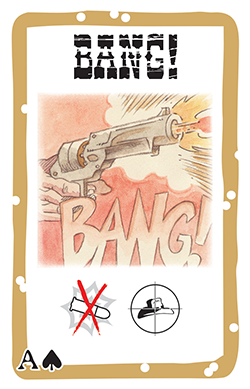
\includegraphics[width=\cardSize\linewidth]{Hnede/01_bang.png}
  \caption[Bang!]{Vyvolá efekt Bang! na hráča na dostrel. Túto kartu možno zahrať len 1-krát za ťah.}
  \label{fig:bang}
\end{minipage}
\hfill
\begin{minipage}[t]{\minipageSize}\centering
  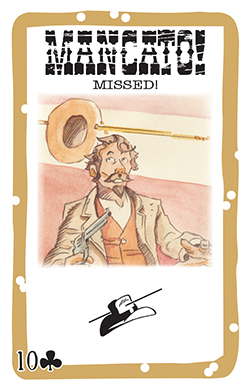
\includegraphics[width=\cardSize\linewidth]{Hnede/01_mancato.png}
  \caption[Vedle!]{Zahraním tejto karty zrušíte efekt Bang!, ktorý mieri na vás.}
  \label{fig:vedle}
\end{minipage}
\hfill
\begin{minipage}[t]{\minipageSize}\centering
  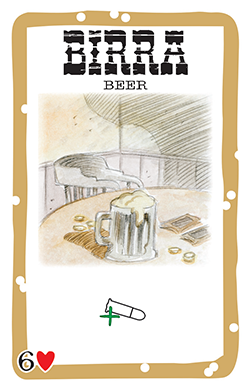
\includegraphics[width=\cardSize\linewidth]{Hnede/01_birra.png}
  \caption[Pivo]{Zahraním tejto karty si hráč doplní 1 život v rámci svojho maxima. Túto kartu možno zahrať aj mimo svojho ťahu, ak hráč utrpel smrteľné zranenie. Ak hráč stratil viac životov naraz, musí zahrať toľko kariet Pivo, aby sa vrátil aspoň na 1 život. Napríklad ak má hráč 2 životy a vybuchne mu Dynamit, musí zahrať 2 karty Pivo. Kartu Pivo nemožno zahrať, ak sú v hre už len poslední 2 hráči.}
  \label{fig:bang}
\end{minipage}
\hfill
\begin{minipage}[t]{\minipageSize}\centering
  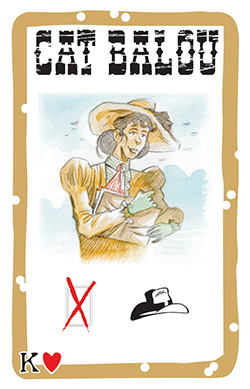
\includegraphics[width=\cardSize\linewidth]{Hnede/01_catbalou.png}
  \caption[Cat Balou]{Zahraním tejto karty hráč môže odhodiť do odhadzovacej kôpky ľubovoľnú kartu z hry (na stole alebo na ruke hráča). Kartu je možné zahrať aj na seba a tak si odhodiť na príklad chrestýša alebo odmenu.}
  \label{fig:duel}
\end{minipage}



\end{figure}

\begin{figure}[!h]

\begin{minipage}[t]{\minipageSize}\centering
  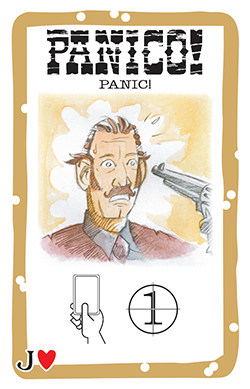
\includegraphics[width=\cardSize\linewidth]{Hnede/01_panico.png}
\caption[Panico!]{Zahraním tejto karty si môžete vziať ľubovoľnú kartu z ruky alebo z hry hráča vo vzdialenosti 1. Túto vzdialenosť ovplyvňujú karty ako Appaloosa a Silver, nie však zbrane vyložené pred hráčom. Kartu možno zahrať aj na seba.}
  \label{fig:panico}
\end{minipage}
\hfill
\begin{minipage}[t]{\minipageSize}\centering
  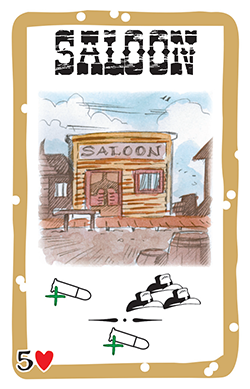
\includegraphics[width=\cardSize\linewidth]{Hnede/01_saloon.png}
  \caption[Saloon]{Zahraním tejto karty získajú všetci živí hráči efekt Pivo. Saloon nie je karta Pivo, preto ho možno zahrať aj v hre dvoch hráčov, ale iba počas vlastného ťahu.}
  \label{fig:vedle}
\end{minipage}
\hfill
\begin{minipage}[t]{\minipageSize}\centering
  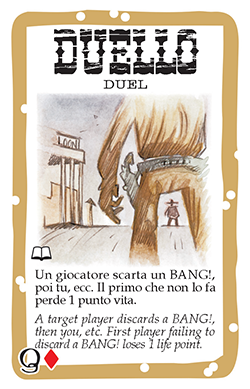
\includegraphics[width=\cardSize\linewidth]{Hnede/01_duello.png}
  \caption[Duel]{Vyzvete ľubovoľného hráča na duel. Hráči sa striedajú v odhadzovaní kariet Bang!. Hráč, ktorý už ďalšiu kartu Bang! neodhodí, stráca 1 život. Začína vyzvaný hráč. Karty Bang! odhodené do duelu sa nepočítajú do limitu Bang!, pretože sa iba odhadzujú, nie hrajú.}
  \label{fig:duel}
\end{minipage}
\hfill
\begin{minipage}[t]{\minipageSize}\centering
  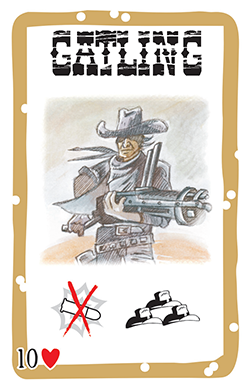
\includegraphics[width=\cardSize\linewidth]{Hnede/01_gatling.png}
  \caption[Guľomet]{Zahraním tejto karty vyvoláte efekt Bang! proti všetkým ostatným hráčom v hre. Nejde o kartu Bang!, takže sa nepočíta do limitu jednej karty Bang! za ťah. Ak niekoho týmto efektom vyradíte, za vyradenie zodpovedáte vy.}
  \label{fig:gatling}
\end{minipage}

\end{figure}




\begin{figure}[!h]
\begin{minipage}[t]{\minipageSize}\centering
  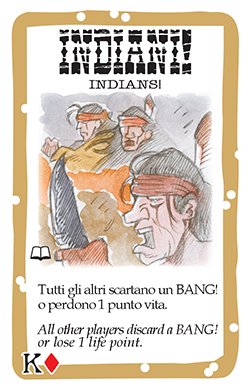
\includegraphics[width=\cardSize\linewidth]{Hnede/01_indiani.png}
 \caption[Indiáni]{Každý hráč okrem toho, kto túto kartu zahral, musí odhodiť kartu Bang!, inak stráca 1 život.}
  \label{fig:bang}
\end{minipage}
\hfill
\begin{minipage}[t]{\minipageSize}\centering
  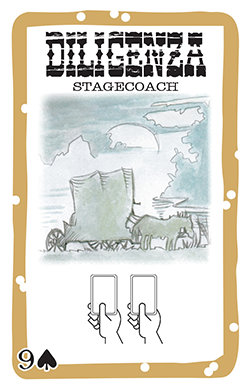
\includegraphics[width=\cardSize\linewidth]{Hnede/01_diligenza.png}
  \caption[Dostavník]{Zahraním tejto karty si hráč potiahne 2 karty.}
  \label{fig:vedle}
\end{minipage}
\hfill
\begin{minipage}[t]{\minipageSize}\centering
  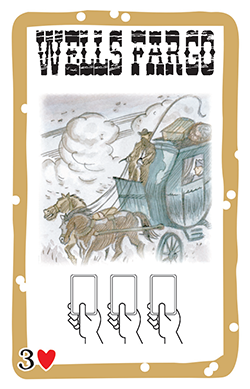
\includegraphics[width=\cardSize\linewidth]{Hnede/01_wellsfargo.png}
  \caption[Wells Fargo]{Zahraním tejto karty si hráč potiahne 3 karty.}
  \label{fig:duel}
\end{minipage}
\hfill
\begin{minipage}[t]{\minipageSize}\centering
  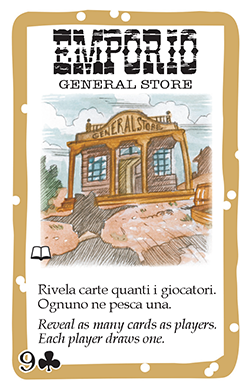
\includegraphics[width=\cardSize\linewidth]{Hnede/01_emporio.png}
\caption[Emporio]{Na stôl sa vyloží (tvárou hore) toľko kariet koľko je hráčov v hre (živí/duch). Každý hráč si zoberie 1 kartu. Začína sa hráčom ktorý túto kartu zahral a postupuje sa po smere hodinových ručičiek.}
  \label{fig:panico}
\end{minipage}
\end{figure}


\begin{comment}
\begin{figure}[!h]
\begin{minipage}[t]{\minipageSize}\centering
  \includegraphics[width=\cardSize\linewidth]{}
 \caption[]{}
  \label{fig:bang}
\end{minipage}
\hfill
\begin{minipage}[t]{\minipageSize}\centering
  \includegraphics[width=\cardSize\linewidth]{}
  \caption[]{}
  \label{fig:vedle}
\end{minipage}
\hfill
\begin{minipage}[t]{\minipageSize}\centering
  \includegraphics[width=\cardSize\linewidth]{}
  \caption[]{}
  \label{fig:duel}
\end{minipage}
\hfill
\begin{minipage}[t]{\minipageSize}\centering
  \includegraphics[width=\cardSize\linewidth]{}
\caption[]{}
  \label{fig:panico}
\end{minipage}
\end{figure}
\end{comment}


\begin{figure}[!h]
\begin{minipage}[t]{\minipageSize}\centering
  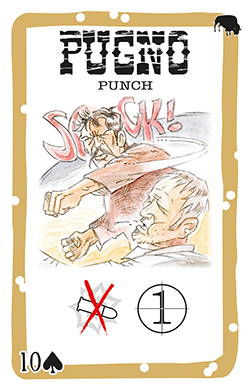
\includegraphics[width=\cardSize\linewidth]{Hnede/03_pugno.png}
 \caption[Punch]{Vyvolá efekt Bang! na hráča vo vzdialenosti 1. Vzdialenosť ovplyvňujú karty vyložené pred hráčmi.}
  \label{fig:bang}
\end{minipage}
\hfill
\begin{minipage}[t]{\minipageSize}\centering
  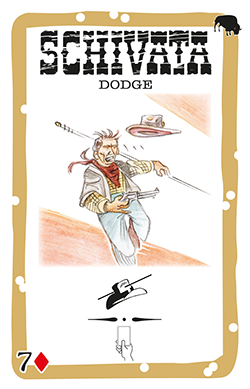
\includegraphics[width=\cardSize\linewidth]{Hnede/03_schivata.png}
  \caption[Úhyb]{Vyvolá efekt Vedle!. Hráč, ktorý túto kartu zahral, si potom potiahne 1 kartu z balíčka.}
  \label{fig:vedle}
\end{minipage}
\hfill
\begin{minipage}[t]{\minipageSize}\centering
  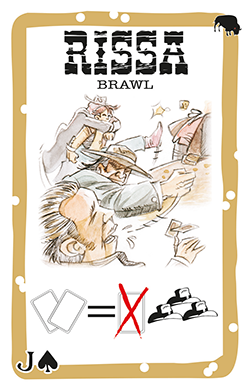
\includegraphics[width=\cardSize\linewidth]{Hnede/03_rissa.png}
  \caption[Rvačka]{Zahraním tejto karty spolu odhodenim ľubovoľnej karty (bez efektu) sa každý hráč stava cieľom efektu Cat Balou.}
  \label{fig:duel}
\end{minipage}
\hfill
\begin{minipage}[t]{\minipageSize}\centering
  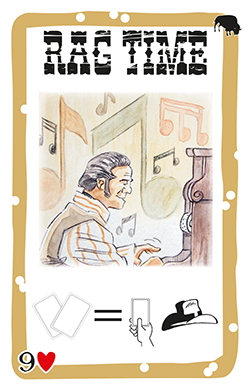
\includegraphics[width=\cardSize\linewidth]{Hnede/03_rag_time.png}
\caption[Rag Time]{Zahraním tejto karty spolu s odhodenim ľubovoľnej karty (bez efektu) sa ľubovoľný hráč bez ohľadu na vzdialenosť stáva cieľom efektu Panika!.}
  \label{fig:panico}
\end{minipage}
\end{figure}


\begin{figure}[!h]
\begin{minipage}[t]{\minipageSize}\centering
  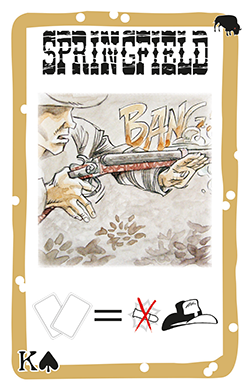
\includegraphics[width=\cardSize\linewidth]{Hnede/03_springfield.png}
 \caption[Springfield]{Zahraním tejto karty a odhodením ľubovoľnej ďalšej karty bez účinku sa ľubovoľný hráč stáva cieľom efektu Bang!.}
  \label{fig:bang}
\end{minipage}
\hfill
\begin{minipage}[t]{\minipageSize}\centering
  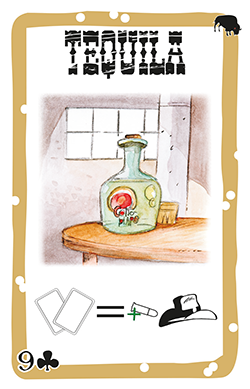
\includegraphics[width=\cardSize\linewidth]{Hnede/03_tequila.png}
  \caption[Tequilla]{Zahraním tejto karty a odhodením ľubovoľnej ďalšej karty bez účinku môžete ľubovoľnému hráčovi, aj sebe, udeliť efekt Pivo. Nejde o kartu Pivo, takže ju možno zahrať aj pri dvoch zostávajúcich hráčoch, ale nikdy nie mimo svojho ťahu.}
  \label{fig:vedle}
\end{minipage}
\hfill
\begin{minipage}[t]{\minipageSize}\centering
  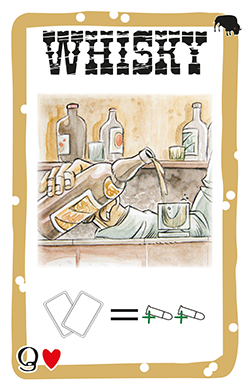
\includegraphics[width=\cardSize\linewidth]{Hnede/03_whisky.png}
  \caption[Whiskey]{Zahraním tejto karty a odhodením ľubovoľnej ďalšej karty bez účinku získate 2 efekty Pivo. Nejde o kartu Pivo, takže ju možno zahrať aj pri dvoch zostávajúcich hráčoch, ale nikdy nie mimo svojho ťahu.}
  \label{fig:duel}
\end{minipage}
\hfill
\begin{minipage}[t]{\minipageSize}\centering
  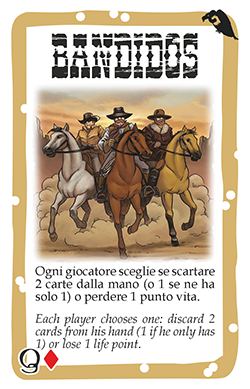
\includegraphics[width=\cardSize\linewidth]{Hnede/07_bandidos.png}
\caption[Divoká Banda]{Každý hráč okrem toho, kto túto kartu zahral, odhodí z ruky 2 karty alebo 1 kartu Bang!. Ak má hráč v ruke len 1 kartu, odhodí ju bez ďalšej penalizácie. Hráča bez kariet sa tento efekt netýka.}
  \label{fig:panico}
\end{minipage}
\end{figure}

\begin{figure}[!h]
\begin{minipage}[t]{\minipageSize}\centering
  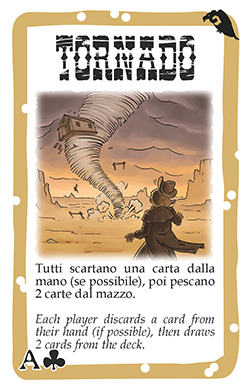
\includegraphics[width=\cardSize\linewidth]{Hnede/07_tornado.png}
 \caption[Tornádo]{Každý hráč dá 2 karty (alebo koľko sa mu dá) hráčovi po svojej ľavici. Výmena musí prebehnúť naraz. Teda hráč nemôže posunúť daľšiemu hráčovi karty ktoré práve dostal od hráča po svojej pravici.}
  \label{fig:bang}
\end{minipage}
\hfill
\begin{minipage}[t]{\minipageSize}\centering
  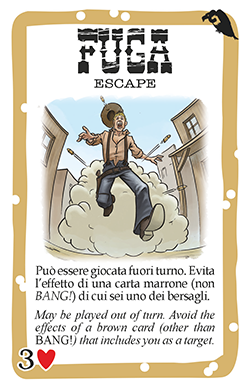
\includegraphics[width=\cardSize\linewidth]{Hnede/07_fuga.png}
  \caption[Útek]{Zahraním tejto karty sa môžete vyhnúť efektu karty, ktorá nie je kartou Bang!. Útek funguje aj proti kartám a efektom zasahujúcim viacerých hráčov, napr. Guľometu alebo Indiánom, ale zruší ich iba vo vzťahu k vám. Útek možno použiť aj proti kartám Väzenie, Dvojitá rána, Opětovná palba, Punch a podobne, nie však proti kartám Roztříštená kulka alebo Dynamit.}
  \label{fig:vedle}
\end{minipage}
\hfill
\begin{minipage}[t]{\minipageSize}\centering
  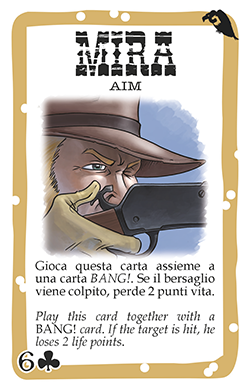
\includegraphics[width=\cardSize\linewidth]{Hnede/07_mira.png}
  \caption[Dvojitá rána]{Zahraním tejto karty spolu s kartou Bang! môžete hráčovi na dostrel odobrať 2 životy. Na vyhnutie sa stačí 1 efekt Vedle!. Táto karta sa počíta do limitu Bang!.}
  \label{fig:duel}
\end{minipage}
\hfill
\begin{minipage}[t]{\minipageSize}\centering
  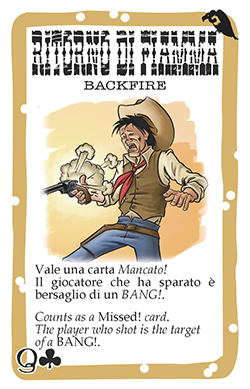
\includegraphics[width=\cardSize\linewidth]{Hnede/07_ritornodifiamma.png}
\caption[Opětovná palba]{Táto karta vyvolá efekt Vedle!; útočiaci hráč sa zároveň stáva cieľom efektu Bang!. Platí aj proti Kulometu, Houfnici a schopnosti postavy Henry Block.}
  \label{fig:panico}
\end{minipage}
\end{figure}


\begin{figure}[!h]
\begin{minipage}[t]{\minipageSize}\centering
  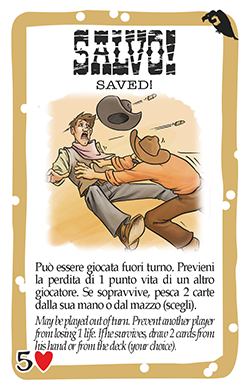
\includegraphics[width=\cardSize\linewidth]{Hnede/07_salvo.png}
 \caption[Obětavý skok]{Zahraním tejto karty zabránite hráčovi stratiť 1 život. Ak tým zachránite hráča pred vyradením, potiahne si 2 náhodné karty z ruky zachráneného hráča. Ak takto zachránite Henryho Blocka pred smrteľnou ranou, útočiaci hráč sa stáva cieľom efektu Bang!. Podľa dohody pri stole platí, že pri výbuchu Dynamitu, ktorý by hráča dostal do mínusových životov, nemožno kartu Obětavý skok zahrať.}
  \label{fig:bang}
\end{minipage}
\hfill
\begin{minipage}[t]{\minipageSize}\centering
  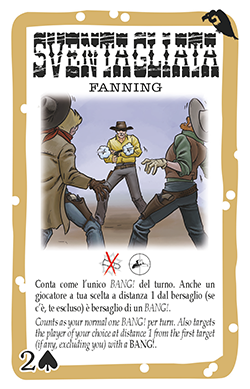
\includegraphics[width=\cardSize\linewidth]{Hnede/07_sventagliata.png}
  \caption[Roztříštená kulka]{Účinkuje ako karta Bang! na dostrel a počíta sa do limitu Bang!. Hráč podľa vášho výberu vo vzdialenosti 1 od primárneho cieľa sa zároveň stáva cieľom efektu Bang!. Túto vzdialenosť ovplyvňujú karty vyložené pred hráčmi. \\
  Pr. 1: Vystrelíte na primárny cieľ a sekundárny cieľ má Mustanga. Sekundárny cieľ sa nestáva cieľom dodatočného efektu Bang!.\\
  Pr. 2: Tá istá situácia, no primárny cieľ má pred sebou Silver. Vtedy sa sekundárny cieľ stáva cieľom efektu Bang!.}
  \label{fig:vedle}
\end{minipage}
\hfill
\begin{minipage}[t]{\minipageSize}\centering
  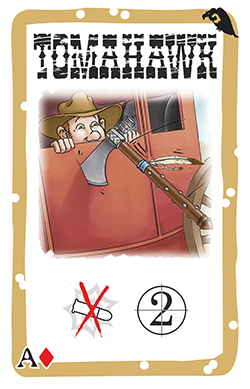
\includegraphics[width=\cardSize\linewidth]{Hnede/07_tomahawk.png}
  \caption[Tomahawk]{Vyvolá efekt Bang! na hráča vo vzdialenosti najviac 2. Túto vzdialenosť ovplyvňujú karty vyložené pred hráčmi, takže Tomahawk možno použiť aj na cieľ vo vzdialenosti 1.}
  \label{fig:duel}
\end{minipage}
\hfill
\begin{minipage}[t]{\minipageSize}\centering
  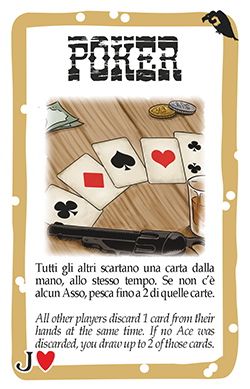
\includegraphics[width=\cardSize\linewidth]{Hnede/07_poker.png}
\caption[Poker]{Všetci ostatní hráči vyložia jednu kartu tvárou dolu. Ak sa medzi kartami nenachádza Eso, hráč si z vyložených kariet zoberie 2 a ostatné sa odhodia. V opačnom prípade si hráč neberie žiadnu kartu.}
  \label{fig:panico}
\end{minipage}
\end{figure}

\begin{figure}[!h]
\begin{minipage}[t]{\minipageSize}\centering
  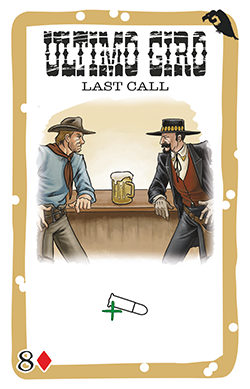
\includegraphics[width=\cardSize\linewidth]{Hnede/07_ultimogiro.png}
 \caption[Posledné pivo]{Zahraním tejto karty získate efekt Pivo.}
  \label{fig:bang}
\end{minipage}
\hfill
\begin{minipage}[t]{\minipageSize}\centering
  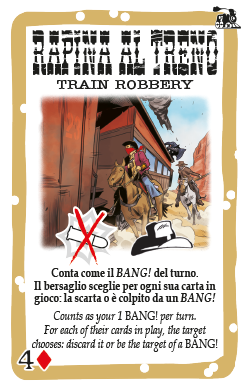
\includegraphics[width=\cardSize\linewidth]{Hnede/33_TrainRobberyA.png}
  \caption[Vlaková loupež]{Zahraním tejto karty proti ľubovoľnému hráčovi vyvoláte toľko samostatných efektov Bang!, koľko má tento hráč kariet v ruke. Každý jednotlivý efekt sa vyhodnocuje osobitne: hráč môže stratiť život, zahrať kartu Vedle!, ťahať na Barel alebo použiť schopnosť postavy, napr. Jourdonnais. Táto karta sa počíta do limitu Bang!.}
  \label{fig:vedle}
\end{minipage}
\hfill
\begin{minipage}[t]{\minipageSize}\centering
  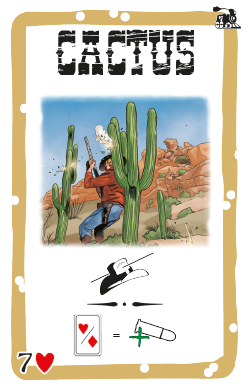
\includegraphics[width=\cardSize\linewidth]{Hnede/34_Cactus.png}
  \caption[Cactus]{Vyvolá efekt Vedle!. Potom otočíte vrchnú kartu balíčka; ak je červená, získate efekt Pivo. Nejde pritom o kartu Pivo, ale iba o efekt Pivo.}
  \label{fig:duel}
\end{minipage}
\hfill
\begin{minipage}[t]{\minipageSize}\centering
  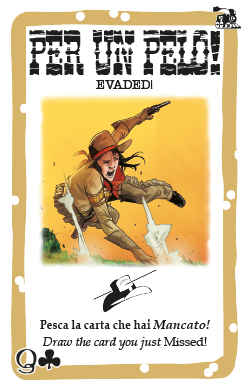
\includegraphics[width=\cardSize\linewidth]{Hnede/35_Evaded.png}
\caption[K zemi!]{Hráč si vezme kartu, proti ktorej práve použil efekt Vedle!. Platí to aj proti Vlakovej loupeži. Pri vyhnutí sa karte Knife Revolver sa najprv vyhodnotí, či sa táto karta vracia útočníkovi do ruky.}
  \label{fig:panico}
\end{minipage}
\end{figure}


\begin{figure}[!h]
\begin{minipage}[t]{\minipageSize}\centering
  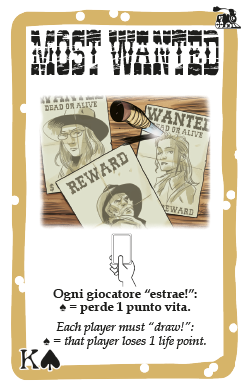
\includegraphics[width=\cardSize\linewidth]{Hnede/36_MostWanted.png}
 \caption[Nejhladanejší]{Každý hráč vrátane toho, kto túto kartu zahral, ťahá vrchnú kartu balíčka. Ak je karta piková, stratí 1 život. Ak by boli takto vyradení všetci hráči naraz, vyhrávajú banditi.}
\end{minipage}
\hfill
\begin{minipage}[t]{\minipageSize}\centering
  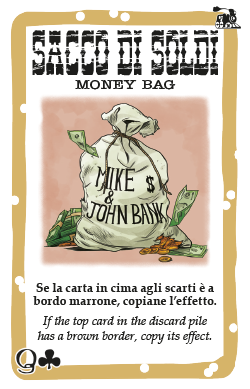
\includegraphics[width=\cardSize\linewidth]{Hnede/38_MoneyBag.png}
 \caption[Pytel peňez]{Ak je na vrchu odhadzovacej kopy hnedá karta, zahraním tejto karty skopírujete jej efekt. Túto kartu nemožno zahrať mimo svojho ťahu.}
\end{minipage}
\hfill
\begin{minipage}[t]{\minipageSize}\centering
  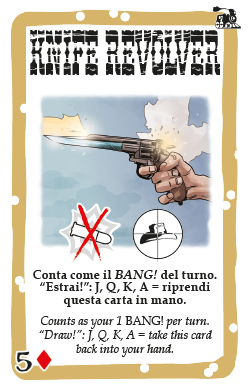
\includegraphics[width=\cardSize\linewidth]{Hnede/37_KnifeRevolver.png}
 \caption[Revolver s nožem]{Vyvolá efekt Bang!. Po zahraní otočíte vrchnú kartu balíčka; ak má hodnotu J, Q, K alebo A, vrátite si kartu Revolver s nožem späť do ruky.}
\end{minipage}
\hfill
\begin{minipage}[t]{\minipageSize}\centering
  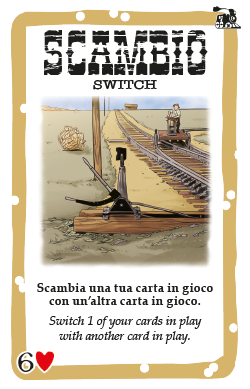
\includegraphics[width=\cardSize\linewidth]{Hnede/31_Switch.png}
 \caption[Výhybka]{Zahraním tejto karty môžete vymeniť svoju kartu v hre za jednu kartu v hre iného hráča. Ak získate novú zbraň, svoju pôvodnú zbraň musíte odhodiť. Nemôžete takto získať kartu s rovnakým názvom, ak ju už máte v hre. Karty, ktoré práve tvoria vlak, sa nepovažujú za karty v hre, a preto ich takto vymeniť nemožno.}
\end{minipage}
\end{figure}

\begin{figure}[!h]
\begin{minipage}[t]{\minipageSize}\centering
  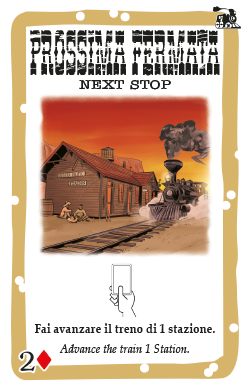
\includegraphics[width=\cardSize\linewidth]{Hnede/40_NextStopA.png}
 \caption[Příští stanice]{Posuňte vlak o 1 stanicu dopredu. Ak týmto efektom vlak dôjde na koniec trate, potiahnete si 1 kartu ešte pred vyhodnotením efektu lokomotívy.}
\end{minipage}
\hfill
\begin{minipage}[t]{\minipageSize}\centering
  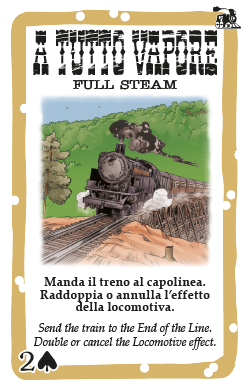
\includegraphics[width=\cardSize\linewidth]{Hnede/39_FullSteam.png}
 \caption[Plnou parou vpřed]{Posuňte vlak rovno na koniec trate a potom sa rozhodnite, či sa efekt lokomotívy nevyhodnotí vôbec, alebo sa vyhodnotí dvakrát za sebou pre všetkých hráčov.}
\end{minipage}
\hfill
\begin{minipage}[t]{\minipageSize}\centering
  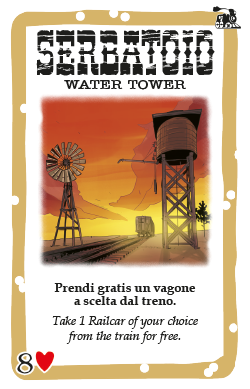
\includegraphics[width=\cardSize\linewidth]{Hnede/32_WaterTower.png}
 \caption[Vodojem]{Zahraním tejto karty získate 1 ľubovoľný vagón zadarmo. V rámci tohto efektu nemožno najprv posúvať vlak. Takto získaný vagón sa nepočíta do bežného limitu vagónov za ťah.}
\end{minipage}
\end{figure}
